% !TEX root = ../../phdthesis_tawatr.tex 

%% ==== ==== ==== ==== 
\section[Galvanic distortion]{Galvanic distortion}\label{sect:galvanic_distortion}

%	\begin{itemize}
%		\item \red{Introductory p.}
%		\item
		 Galvanic distorion is the alteration of electric field due to near-surface small-scale heterogeneity.  
%		\item
		 In theory, the distortion of the MT data may be both galvanic and inductive, but we can choose a proper period range so that only the galvanic distortion is considered \citep{groom1992a, utada2000a}.
%		\item
		 In contrast to marine cases, most of on-land MT observations suffer from galvanic distortion. 
%		\item
		 This section provides the physical principle of galvanic distortion, its mathematical formulation, and the galvanic distortion model or parameterization used in this work.
%	\end{itemize}
	
\begin{figure}[!h]
	\centering
	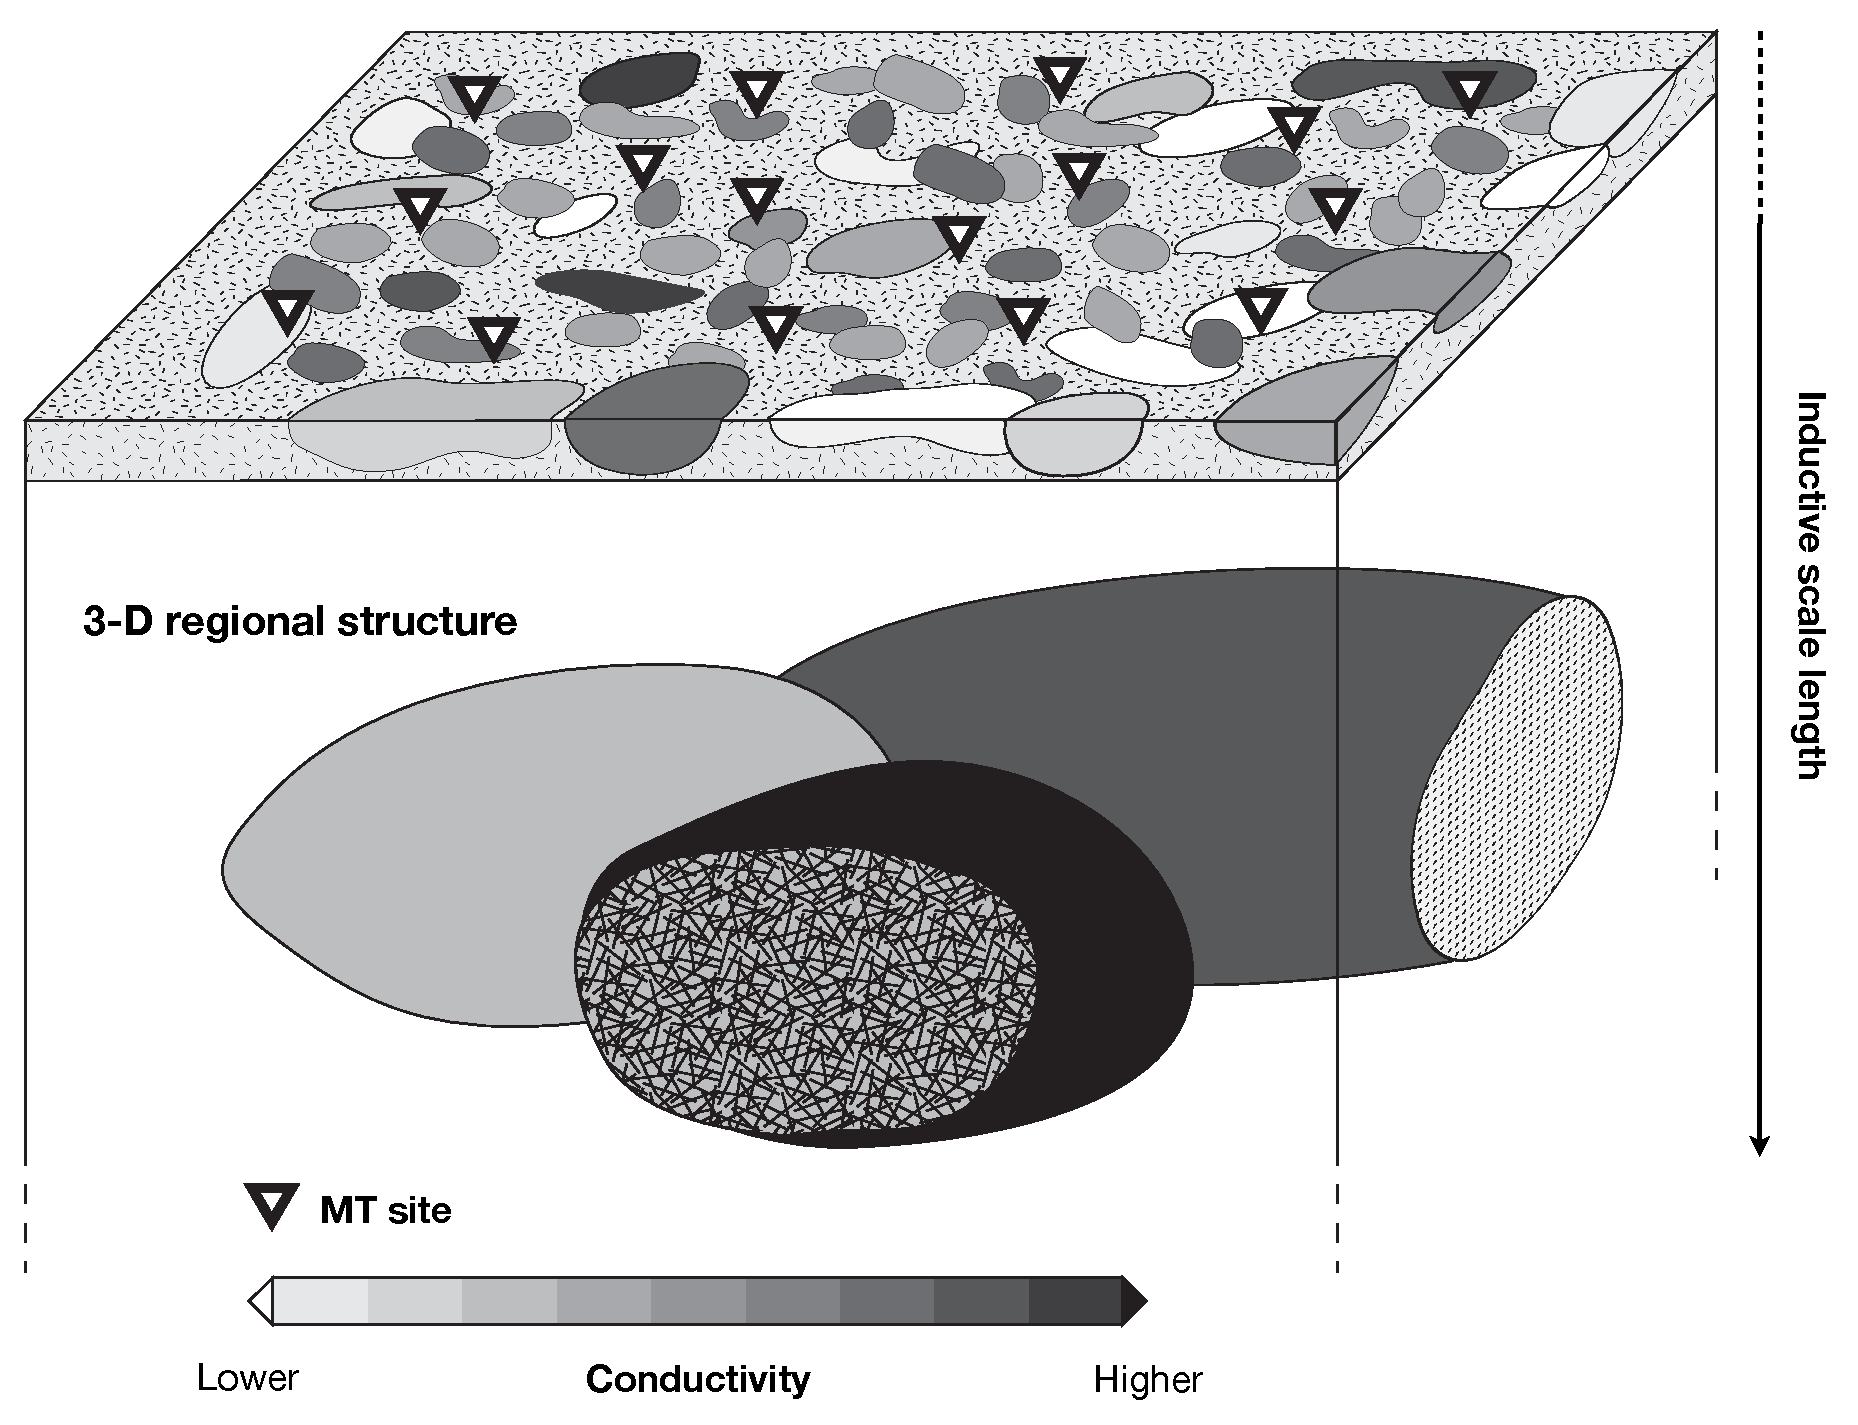
\includegraphics[width=5in]{\figdir/galvanicdistortion_model.pdf}
	\caption[A model of galvanic distortion in this study]{A model of galvanic distortion in this study. The model consists of 3D regional scale structure, which is of interest, and small-scale heterogeneities confined in the near-surface layer, which is shallower and thinner than the inductive scale length of interest \citep[after][]{utada2000a, rung-arunwan2016a}.}
	\label{fig:galvanic_distortion_model}
\end{figure}

%% ==== ==== ==== ==== 
\subsection{Galvanic distortion principle}
		% Theory of galvanic distortion
%	\begin{itemize}
%		\item 
		Following the formulation presented in \citet{groom1992a}; \citet{chave1994a} and \citet{utada2000a},
		this section provides the galvanic distortion principle based on electromagnetic scattering theory, which will leads to the mathematical representation of galvanic distortion.
		
%		\item 
		According to \citet{hohmann1975a}, the electric field observed at an arbitrary position $\rbf$, both internal and external to the scatterer, from a 3D heterogeneous medium can be expressed as
			\begin{equation} \label{eq:efield_int}
				\begin{split}
					\Ebf\fxr & = \Ebf_\Regional\fxr - i\omega\mu_0\sum_j\int_{V_j}  \,g(\rbf,\rbf')\,\delta\sigma_j(\rbf')\, \Ebf(\rbf') \, \dwrt V' \\
					& \quad + \nabla\, \frac{1}{\sigma_0}\, \div{\sum_j \int_{V_j} \,g(\rbf,\rbf')\,\delta\sigma_j(\rbf')\, \Ebf(\rbf') \, \dwrt V' },
				\end{split}
			\end{equation}
			where $V_j$ refers to each scattering body.
%			\red{
			Note that the quantities in Eq. \eqref{eq:efield_int} except the conductivity $\sigma_0$ and $\delta\sigma_j$ and the magnetic permeability $\mu_0$ are frequency dependent, but they are implicitly written.
%			}
%			\blueb{I am not sure how put the frequency dependence of these quantities before the equation. Then I put it here.}
			The anomaly conductivity contrast $\delta \sigma_j(\rbf')$ is defined by
			\begin{equation} \delta \sigma_j(\rbf') = \sigma_j(\rbf') - \sigma_0(\rbf'), 
			\end{equation}
			where $\sigma_j$ is the scatterer conductivity and $\sigma_0$  is the background or regional conductivity structure.
			The analytical expression of the Green's function of the uniform Earth is given by
			\begin{equation}
				g(\rbf,\rbf') = \frac{\expe{i\gamma_0 |\rbf-\rbf'|}}{4\pi|\rbf-\rbf'|},
			\end{equation}
			where $\gamma_0=\sqrt{i\omega\mu_0\sigma_0}$. The inductive scale length, or the electromagnetic skin depth, of the uniform background is 
			\begin{equation}\label{eq:idl_background}
				\lambda_0 = \frac{1}{|\Re\,\gamma_0|}.
			\end{equation}
			From the expression of the electric field \eqref{eq:efield_int}, the first term $\Ebf_\Regional\fxr$ is the field from the background structure, and the second and third terms denote the inductive and galvanic field components from each heterogeneity, which depends on size, conductivity contrast and \emph{inverse} distance.			
			But only the inductive term contains the frequency dependent part, which vanishes at long periods. 
			
			The integral solution for the magnetic field could then be obtained by applying Faraday's law to Eq. \eqref{eq:efield_int};
			\begin{equation}\label{eq:bfield_int}
				\Bbf\fxr = \Bbf_\Regional\fxr + \mu_0 \curl \sum_j \int_{V_j} g(\rbf,\rbf')\,\delta\sigma_j(\rbf')\,\Ebf(\rbf')\, \dwrt V', 
			\end{equation}
			In contrast to the electric field, the magnetic field \eqref{eq:bfield_int} contains only the inductive term due to the heterogeneity. The galvanic component vanishes because of the vector calculus identity that the curl of gradient of any scalar function is the zero vector. Therefore, the galvanic effect comes from the electric field only.
			
			% Induction number
			The contribution from each scattering body or distorter could be determined by the induction number $M_j$, 
			\begin{equation}
				M_j = \frac{L_j}{\lambda_j}.
			\end{equation}
			which is the ratio of its horizontal dimension $L_j$ to its inductive scale length 
			\begin{equation}\label{eq:idl_anomaly}
				\lambda_j=1/|\Re\,\gamma_j|,
			\end{equation}
			where $\gamma_j=\sqrt{i\omega\mu_0\delta\sigma_j}$.
%
			The distorters are generally small in size and then have very small induction numbers.
				If these distorters are confined to the near-surface layer, shallower and thinner than the background inductive scale length (Figure \ref{fig:galvanic_distortion_model}), they produce the \emph{visible} galvanic effect. 
			
			% Spatial aliasing
			Ideally, if we  have an infinitely dense MT survey and infinite band of data, all features could be explained by observation \citep{utada2000a}.			
			However, MT data is spatially insufficient because an MT array consisting of a limited number of sites is generally designed at least to cover the target structure with the typical site spacing that is able to resolve the smallest-scale target of interest.
			Therefore, the typical site spacing may be larger than the size of the distorters.
			The galvanic distorters inevitably cause spatial aliasing in MT data, i.e., both interesting and irrelevant structures are included in the observation. Such an effect is called galvanic distortion. 
			As it is impossible to recover original spatial features by using aliased data, the galvanic distorters are regarded as \emph{unresolvable} structure \citep{booker2014a}. In order to obtain the reliable results, some treatments or augmented approaches to handle the galvanic distortion are essential.
		
%		\red{HU CORRECTION UP TO HERE}
				
		% Draw the conclusion how it becomes real operator
%	\begin{itemize}
%			\item 
			The electric field solution in Eq. \eqref{eq:efield_int} could be simplified as 
			\begin{equation}\label{eq:efield_model}
				\Ebf\fxr = \Ebf_\Regional\fxr + \mbf{e}_\text{I}\fxr + \mbf{e}_\text{G}\fxr,
			\end{equation}
			where $\mbf{e}_\text{I}\fxr$ and $\mbf{e}_\text{G}\fxr$ represent the inductive and galvanic contributions from the scatterer. In the galvanic limit, Eq. \eqref{eq:efield_model} becomes
			\begin{equation}\label{eq:efield_model_approx}
				\Ebf\fxr \approx  \Ebf_\Regional\fxr  + \mbf{e}_\text{G}\fxr
			\end{equation}
			When the size of each scatterer is sufficiently small, the background electric field can be regarded as uniform inside the scatterer. The horizontal vector of the galvanic field $\mbf{e}_{\text{G},\text{h}}\fxr$ can be related to the undistorted horizontal background electric field $\Ebf_\Regional^\text{h}\fxr$ as
			\begin{equation}
				\mbf{e}_{\text{G},\text{h}}\fxr=\alpha \Ebf_{\Regional,\text{h}}\fxr,
			\end{equation}
			where $\alpha$ is a rank-2 real-valued tensor \citep[see][]{chave1994a}.
			The observed \emph{distorted} electric field (Eq. \ref{eq:efield_model_approx}) then becomes
			\begin{equation}
				\Ebf_\text{h}\fxr =  (\Ibf  + \alpha) \Ebf_{\Regional,\text{h}}\fxr = \Cbf\,\Ebf_{\Regional,\text{h}}\fxr,
			\end{equation}
			where $\Cbf$ is called the distortion operator, which is rank-2 real-valued tensor.
						
%	\end{itemize}

			
%		\item 
		Within the scope of galvanic distortion, the distorted impedance tensor is expressed as the product between the distortion operator $\Cbf$ and the regional (undistorted) impedance tensor $\ZbfUndistorted$:
		\begin{equation}\label{eq:z_distorted}
		\begin{split}
			\ZbfDistorted & =\Cbf\ZbfUndistorted, \\
			\ZDistortedMatrix & = \CMatrix\ZMatrixUndistorted \\
				& = \begin{bmatrix} 
						\Cxx\ZxxR + \Cxy\ZyxR & \Cxx\ZxyR + \Cxy\ZyyR \\
						\Cyx\ZxxR + \Cyy\ZyxR & \Cyx\ZxyR + \Cyy\ZyyR
					\end{bmatrix}
		\end{split}
		\end{equation}
		where the distortion operator {\Cbf} is a $2\times2$ matrix, the elements {\Cxx\ \Cxy\ \Cyx\ \Cyy} are real-valued and frequency-independent scalars.


%% ==== Attempts to galvanic distortion	 		 
%\begin{itemize}
%	\item 
	Several attempts have been made to handle the galvanic distortion problem. Here we briefly summarize some of them. The nature of solving the problem of galvanic distortion is an underdetermined problem. Some constraints or assumptions are necessary.
	For example, the tensor decomposition methods \citep[e.g.,][]{groom1989a, chave1994a, smith1995a, mcneice2001a} is viable under the assumption of 2D regional structure.
	\citet{gomez-trevino2014a} proposed the solution with the aid of rotational invariants, but it is limited to 2D.
%	\item
	Ideally, \citet{utada2000a} introduced the constraints from Faraday's law, but it is impractical in reality.
%	\item 
%	\red{
	The phase tensor \citep{caldwell2004a} and the vertical magnetic transfer function galvanic distortion-free solution. However, because of their absence of magnitude, the inversion based on the phase tensor and the vertical magnetic transfer function strongly depends on the starting models \citep{siripunvaraporn2009a, patro2013a, tietze2015a}. 
%	}
	Also, the vertical magnetic transfer function or tipper is another galvanic distortion-free response.
	However, the tipper is only sensitive to the lateral contrast in conductivity. Therefore the model inverted from the tipper relies on an intial or \emph{a priori} model.
%	\item 
%	\red{
%	However, the phase tensor-based inversion would give \citep{tietze2015a}
%	Some people might apply the constraints to the known structures, e.g., ocean, to get more reliable results from the phase-tensor-based inversion. \redb{see Kanda paper}}
%	\redb{Check the paper of Uyeshima and Tietze}
%	\item 
	Simultaneous inversion of MT data and galvanic distortion \citep[e.g.,][]{sasaki2006a, jones2011a, avdeeva2015a} is also a forthcoming approach. However, its implementation is rather complicated and still it does not fully solve the problem.
%\end{itemize}

%% ==== ==== ==== ====
%\subsection
%		Thus the definition of regional scale is different with different frequency range.

%% ==== ==== ==== ====
	\subsection[Groom--Bailey's framework]{Distortion operator parameterization: Groom--Bailey's framework}
%	\begin{itemize}
%		\item
		 The distortion operator $\Cbf$ can be treated in numerous ways. In this work, we adopted the Groom--Baileys' model of galvanic distortion, which is regarded as one of the standard models of galvanic distortion 
\citep[e.g.,][]{ chave1994a, mcneice2001a, chave2012a}.
		Its principle is briefly described as follows.
%		\parencite[e.g.,][]{chave1994a}[ and see also][]{chave2012a}

%		\item
		 Any $2\times2$ real-valued matrices {\Mbf} could be represented by the linear combination of the modifined Pauli spin matrices \citep{spitz1985a},
		\begin{equation}
			\Mbf = \alpha_0\SigmaZero+\alpha_1\SigmaOne+\alpha_2\SigmaTwo + \alpha_3\SigmaThree,
		\end{equation}
		where the coefficients $\alpha_{i=0,...,3}$ are arbitrary constants. The modifined Pauli spin matrices are
		\begin{equation}
			\SigmaZero=\SigmaZeroMat, \quad
			\SigmaOne=\SigmaOneMat, \quad
			\SigmaTwo=\SigmaTwoMat, \quad
			\SigmaThree=\SigmaThreeMat,
		\end{equation}
		which are mutually orthonormal. Based on these basis matrices,
		\citet{groom1989a} proposed a \emph{physically-based} parameterization of the distortion operator \Cbf, which will be referred to as Groom--Bailey's distortion model:
		\begin{equation}\label{eq:c_gtsa}
			\Cbf = \gain\Tbf\Sbf\Abf.
		\end{equation}
		The positive scalar {\gain} is called the site gain.
		By analogy to deformation theory of materials (Figure \ref{fig:gtes_vector}), the matrices {\Tbf}, {\Sbf} and {\Abf} are, respectively, the twist, shear, and splitting (or anisotropy, but later will be referred to splitting only) operators, which are $2\times2$ real-valued matrices. 
		They are given by
		\begin{equation}\label{eq:TSA_def}
			\begin{split}
				\Tbf & = \NT(\SigmaZero+\twistp\SigmaTwo) = \NT\Tmatrix, \\
				\Sbf & = \NS(\SigmaZero+\shearp\SigmaOne) = \NS\Smatrix, \\
				\Abf & = \NA(\SigmaZero+\splittingp\SigmaThree)  = \NA\Amatrix, \\
			\end{split}
		\end{equation}
		where \twistp, {\shearp}, and {\splittingp} are twist, shear, and splitting parameters; {\NT}, {\NS}, and {\NA} are the normalizing coefficients defined from the Frobenius norm of each distortion operator \citep[also see][]{bibby2005a}:
		\begin{equation}
				\NT = \frac{1}{\sqrt{1+t^2}}, \quad
				\NS = \frac{1}{\sqrt{1+e^2}}\quad \text{ and } \quad
				\NA = \frac{1}{\sqrt{1+s^2}}. 
		\end{equation}
		These normalizing coefficients are introduced to ensure that the power of the distorted electric fields is conserved.  
		
%		\item 
		The twist and shear parameters, {\twistp} and {\shearp}, can be physically represented by the twist and shear angles:
		\begin{equation}
			\begin{split}
				\twistp & = \tan \twista \\
				\shearp & = \tan \sheara 
			\end{split}
		\end{equation}

%% ==== Figure distored electric field vectors
\begin{figure}[!h]
	\centering
	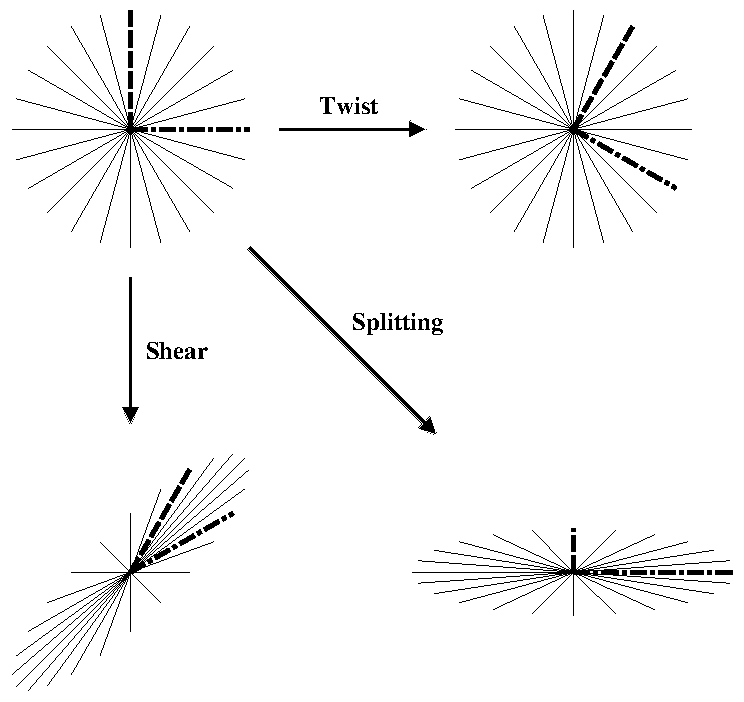
\includegraphics[width=4in]{\figdir/plot_uvec_crop.pdf}
	\caption[Effect of twist, shear and anisotropy operators on a family of unity vectors]{Effect of twist, shear and anisotropy operators on a family of unity vectors, where the twist shear and splitting parameters are $\tan 30^\circ$ \citep[after][]{groom1989a}.}
	\label{fig:gtes_vector}
	% Sketch to illustrate the effects of twist, shear and anisotropy. On the top is a group of unity vectors with 2 reference vectors in red and blue. On the bottom are the groups of vectors after application of (from left to right) twist (Eq. 2.114), shear (Eq. 2.113) and atnisotropy (Eq. 2.112). The black dashed lines indicate the original position and length of the two reference vectors (red and blue), which are now delocated and/or deformed. Redrawn from Groom (1988) and Groom and Bailey (1989).
\end{figure}
		
%		\item 
		By substituting the definitions of twist, shear, and splitting operators (Eq. \ref{eq:TSA_def}) into Eq. \eqref{eq:c_gtsa}, the explicit form of the distortion operator $\Cbf$ in terms of Groom--Bailey's distortion parameters is:		
		\begin{equation}\label{eq:c_gb}
			\Cbf = \CMatrix = \gain\NT\NS\NA\begin{bmatrix} (1+\splittingp)(1-\twistp\shearp) & (1-\splittingp)(\shearp-\twistp) \\
(1+\splittingp)(\shearp+\twistp) & (1-\splittingp)(1+\twistp\shearp) \end{bmatrix}.
		\end{equation}
		The distorted impedance could be calculated by substituting the distortion operator as expressed in Eq. \eqref{eq:c_gb} into Eq. \eqref{eq:z_distorted}.
%		\item 
		We can also write the the distortion operator $\Cbf$ as a linear combination of the modified Pauli spin matrices:
		\begin{equation}
			\Cbf = \cZero \SigmaZero + \cOne \SigmaOne + \cTwo\SigmaTwo + \cThree\SigmaThree,
		\end{equation}	
		where the coefficients $c_i$ are:
		\begin{equation}\label{eq:alphai_gb}
		\begin{split}
			\cZero & = \gain\, \NT\NS\NA\,(1-\shearp\splittingp\twistp), \\
			\cOne & = \gain\, \NT\NS\NA\,(\shearp+\splittingp\twistp), \\
			\cTwo & = \gain\, \NT\NS\NA\,(\shearp\splittingp+\twistp), \\
			\cThree & = \gain\, \NT\NS\NA\,(\splittingp-\shearp\twistp). \\
		\end{split}
	\end{equation}
%\gain\, \NT(\SigmaZero+\twistp\SigmaTwo) \, \NS(\SigmaZero+\shearp\SigmaOne) \, \NA(\SigmaZero+\splittingp\SigmaThree) \\
%			& =  \gain\, \NT\NS\NA\,( (1-\shearp\twistp\splittingp)\SigmaZero+(\shearp+\splittingp\twistp)\SigmaOne + (\twistp+\shearp\splittingp)\SigmaTwo + (\splittingp-\shearp\twistp)\SigmaThree) \\				

%		\item 
		It is also important to note that the distortion operators -- $\gain, \Tbf, \Abf$ and $\Sbf$ -- act differently on the impedance tensors (Figure \ref{fig:gtes_vector}). The site gain $\gain$ is a scalar. Hence the magnitude of the impedance tensor will be scaled up or down. The effect of site gain {\gain} is then called the \emph{static shift} -- frequency independent variation in the magnitude, or apparent resistivity, MT data. The twist, shear, and splitting operators, cause the geometrical change, changing the dimensionality of the impedance tensor, and the mixing among components of impedance tensor or called \emph{phase mixing}.
%		\textcolor{red}{[Citation for phase mixing]}. 
%	\end{itemize}



	
